\documentclass[11pt]{article}

\usepackage[letterpaper,margin=0.85in]{geometry}
\usepackage{microtype}
\usepackage{xcolor}
\usepackage[scaled=0.92]{helvet}
\usepackage{tikz}
\usepackage{enumitem}
\usepackage{booktabs}
\usepackage{caption}
\usetikzlibrary{positioning, fit, backgrounds, calc,
                arrows.meta, shapes.geometric, decorations.pathreplacing}

% ---- Palette: Paul Tol bright ----------------------------------------
\definecolor{bus48v} {HTML}{EE6677}
\definecolor{bus12v} {HTML}{228833}
\definecolor{bus5v}  {HTML}{4477AA}
\definecolor{buseth} {HTML}{66CCEE}
\definecolor{buscan} {HTML}{CCBB44}
\definecolor{buspcie}{HTML}{AA3377}
\definecolor{busgmsl}{HTML}{EE7733}
\definecolor{bususb} {HTML}{332288}

% ---- Subsystem pane tints (very pale) --------------------------------
\definecolor{zoneA}{HTML}{F4E8E8}   % power      — pale warm
\definecolor{zoneB}{HTML}{E8EEF6}   % compute    — pale blue
\definecolor{zoneC}{HTML}{EAF1EA}   % motor      — pale green
\definecolor{zoneD}{HTML}{F8EFE6}   % sensing    — pale orange

\tikzset{
  >={Stealth[length=2.0mm, width=1.4mm]},
  block/.style={
    draw=black!55, line width=0.6pt, rounded corners=2pt,
    rectangle, minimum height=10mm, minimum width=22mm,
    align=center, inner sep=3pt,
    fill=white,
    font=\sffamily\footnotesize, text=black!85
  },
  blocksm/.style={
    draw=black!55, line width=0.6pt, rounded corners=2pt,
    rectangle, minimum height=10mm, minimum width=16mm,
    align=center, inner sep=3pt,
    fill=white,
    font=\sffamily\footnotesize, text=black!85
  },
  motor/.style={
    draw=black!55, line width=0.6pt, circle, minimum size=9mm,
    align=center, fill=white,
    font=\sffamily\footnotesize, text=black!85
  },
  pblock/.style={
    draw=black!55, line width=0.6pt, rounded corners=2pt,
    rectangle, minimum height=11mm, minimum width=26mm,
    align=center, inner sep=3pt, fill=white,
    font=\sffamily\footnotesize, text=black!85
  },
  fuse/.style={
    draw=black!55, line width=0.6pt, rounded corners=1pt,
    rectangle, minimum height=8mm, minimum width=4mm, fill=white
  },
  term/.style={
    draw=black!55, line width=0.6pt, circle, minimum size=2mm,
    inner sep=0pt, fill=white
  },
  zonelabel/.style={
    font=\sffamily\bfseries\scriptsize, text=black!55, inner sep=0pt
  },
  zone/.style={
    draw=black!18, line width=0.4pt, rounded corners=4pt,
    inner sep=5mm
  },
  buswire/.style={
    line width=1.0pt, line cap=round, line join=round,
    rounded corners=2.5pt
  },
  pwire/.style={
    line width=0.8pt, line cap=round, line join=round,
    rounded corners=2pt, draw=black!70
  },
}

\setlist{nosep, leftmargin=*}

\begin{document}

\section*{Electrical Design}

\subsection*{4.1 Overview}
The 2026 electrical architecture is organised into four subsystems: power
distribution, network and computation, sensing, and motor control.
Figure~\ref{fig:electrical-block} shows how these subsystems interconnect.

\begin{itemize}
  \item \textbf{Power} — a 48~V battery feeds two buck converters (12~V and 5~V
    rails) that supply the rest of the vehicle (Section~4.2).
  \item \textbf{Compute} — a Jetson Orin GPU handles perception and high-level
    control. It commands a Teensy~4.1 microcontroller over USB serial
    (Section~4.5).
  \item \textbf{Sensing} — three ZED~X stereo cameras, a Velodyne LiDAR, and an
    Xsens GPS feed the Jetson (Section~4.4).
  \item \textbf{Motor control} — the Teensy runs a closed-loop controller and
    commands two SPARK~MAX motor controllers over CAN, which in turn drive
    two NEO brushless motors (Section~4.3).
\end{itemize}

The emergency-stop circuit is implemented in hardware: it directly interrupts
the supply to both SPARK~MAX controllers, immediately removing torque from
both motors regardless of software state.

\begin{figure}[h]
\centering
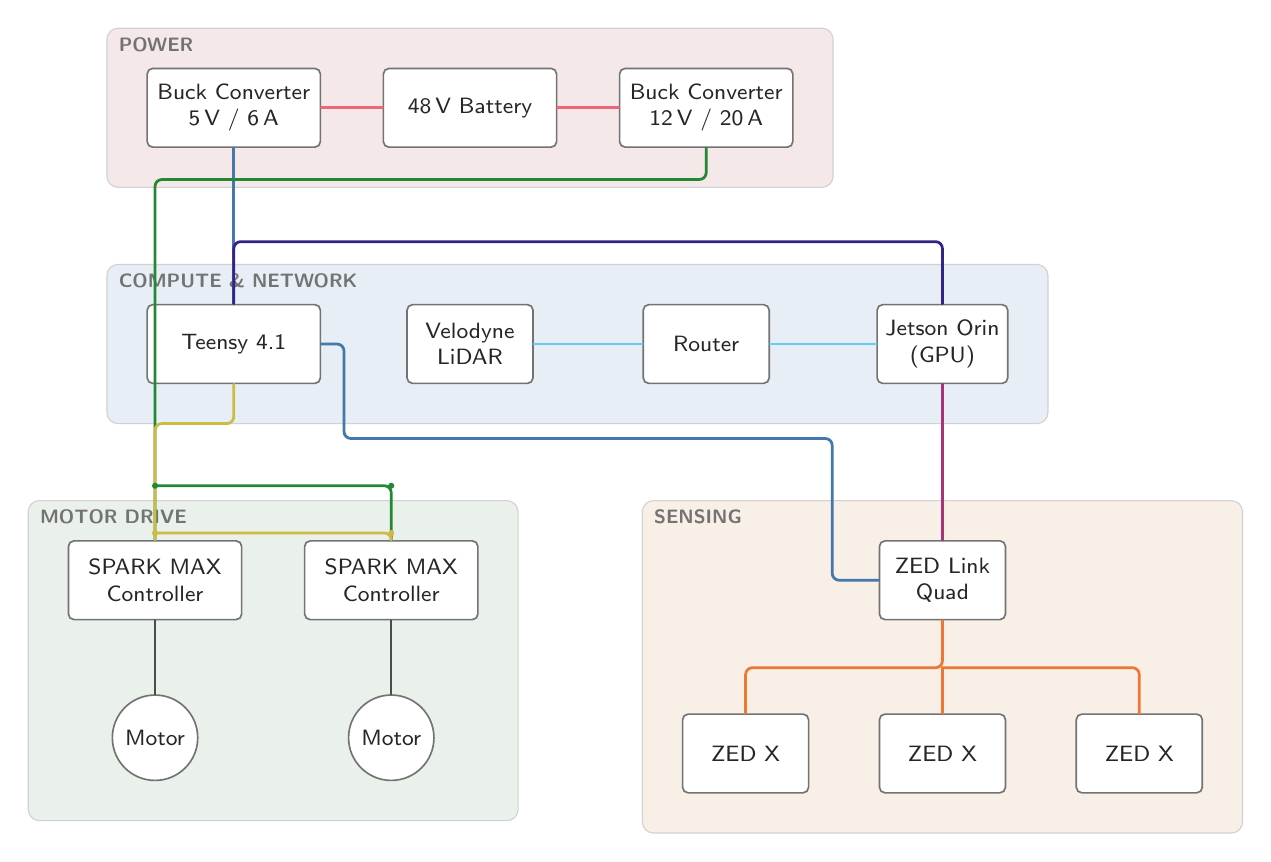
\begin{tikzpicture}[x=1cm, y=1cm]

% ---- Layout philosophy ---------------------------------------------
% Compute hub spreads across the middle row so each downstream connection
% drops straight down with no horizontal trunk crossings. Trunks in the
% gap below row 2 each get their own y-channel (>=4 mm apart).
%
%   Row 1 (y=0):     Power
%   Row 2 (y=-3):    Compute hub (Teensy | Velodyne | Router | Jetson)
%   Row 3 (y=-6):    Drives + sensor aggregator
%   Row 4 (y=-8):    Motors + cameras
%
% Trunk channels in gap:
%   y=-4.2  5V  (Teensy -> ZED Link Quad)
%   y=-4.8  12V (Buck12 -> SPARK MAX trunk)
%   y=-5.4  CAN (Teensy -> SPARK MAX trunk)

% ---- Nodes ---------------------------------------------------------
% Row 1: power
\node[block] (buck5)    at (-3.0, 0)    {Buck Converter\\5\,V / 6\,A};
\node[block] (battery)  at ( 0.0, 0)    {48\,V Battery};
\node[block] (buck12)   at ( 3.0, 0)    {Buck Converter\\12\,V / 20\,A};

% Row 2: compute hub (CAN dropped — represented as a labeled trunk)
\node[block]   (teensy)   at (-3.0, -3.0) {Teensy 4.1};
\node[blocksm] (velodyne) at ( 0.0, -3.0) {Velodyne\\LiDAR};
\node[blocksm] (router)   at ( 3.0, -3.0) {Router};
\node[blocksm] (jetson)   at ( 6.0, -3.0) {Jetson Orin\\(GPU)};

% Row 3: drives + sensor aggregator
\node[block]   (sparkL)   at (-4.0, -6.0) {SPARK MAX\\Controller};
\node[block]   (sparkR)   at (-1.0, -6.0) {SPARK MAX\\Controller};
\node[blocksm] (zedlink)  at ( 6.0, -6.0) {ZED Link\\Quad};

% Row 4: actuators + cameras
\node[motor]   (motorL) at (-4.0, -8.0) {Motor};
\node[motor]   (motorR) at (-1.0, -8.0) {Motor};
\node[blocksm] (cam1) at ( 3.5, -8.2) {ZED X};
\node[blocksm] (cam2) at ( 6.0, -8.2) {ZED X};
\node[blocksm] (cam3) at ( 8.5, -8.2) {ZED X};

% ---- Subsystem panes (background) ---------------------------------
\begin{scope}[on background layer]
  \node[zone, fill=zoneA, fit=(buck5)(battery)(buck12)] (z_power) {};
  \node[zone, fill=zoneB, fit=(teensy)(velodyne)(router)(jetson)] (z_compute) {};
  \node[zone, fill=zoneC, fit=(sparkL)(sparkR)(motorL)(motorR)] (z_motor) {};
  \node[zone, fill=zoneD, fit=(zedlink)(cam1)(cam2)(cam3)] (z_sensing) {};
\end{scope}

\node[zonelabel, anchor=north west] at ($(z_power.north west)   + (1.5mm,-1.2mm)$) {POWER};
\node[zonelabel, anchor=north west] at ($(z_compute.north west) + (1.5mm,-1.2mm)$) {COMPUTE \& NETWORK};
\node[zonelabel, anchor=north west] at ($(z_motor.north west)   + (1.5mm,-1.2mm)$) {MOTOR DRIVE};
\node[zonelabel, anchor=north west] at ($(z_sensing.north west) + (1.5mm,-1.2mm)$) {SENSING};

% ---- Wires --------------------------------------------------------
% 48V (short horizontals between battery and bucks)
\draw[buswire, color=bus48v] (buck5.east)   -- (battery.west);
\draw[buswire, color=bus48v] (battery.east) -- (buck12.west);

% 5V: Buck5 -> Teensy (straight down through the gap)
\draw[buswire, color=bus5v] (buck5.south) -- (teensy.north);

% 5V trunk: Teensy.east -> channel y=-4.2 -> ZED Link Quad.west
% drops in the gap just east of Teensy, runs in its own channel,
% comes up into the left side of ZED Link Quad.
\coordinate (t5_drop) at (-1.6, -3.0);    % just east of Teensy
\coordinate (t5_chan) at (-1.6, -4.2);    % drop into 5V channel
\coordinate (t5_up)   at ( 4.6, -4.2);    % rise point west of ZED Link Quad
\draw[buswire, color=bus5v]
  (teensy.east) -- (t5_drop) -- (t5_chan) -- (t5_up) |- (zedlink.west);

% 12V trunk: Buck12.south -> channel y=-4.8 -> sparkL.north and sparkR.north
\coordinate (p12_in)   at ($(buck12.south) + (0,-0.4)$);
\coordinate (p12_chL)  at (sparkL |- 0,-4.8);
\coordinate (p12_chR)  at (sparkR |- 0,-4.8);
\draw[buswire, color=bus12v]
  (buck12.south) -- (p12_in) -| (p12_chL) -- (sparkL.north);
\draw[buswire, color=bus12v]
  (p12_chL) -- (p12_chR) -- (sparkR.north);

% ETH (Router <-> Velodyne, Router <-> Jetson)
\draw[buswire, color=buseth] (velodyne.east) -- (router.west);
\draw[buswire, color=buseth] (router.east)   -- (jetson.west);

% USB serial: Jetson -> top channel -> Teensy
\coordinate (usb_chT) at (teensy |- 0,-1.7);
\coordinate (usb_chJ) at (jetson |- 0,-1.7);
\draw[buswire, color=bususb] (jetson.north) -- (usb_chJ) -- (usb_chT) -- (teensy.north);

% CAN trunk: Teensy.south -> channel y=-5.4 -> both SPARK MAX (multi-drop)
\coordinate (can_drop) at ($(teensy.south) + (0,-0.5)$);
\coordinate (can_chL)  at (sparkL |- 0,-5.4);
\coordinate (can_chR)  at (sparkR |- 0,-5.4);
\draw[buswire, color=buscan]
  (teensy.south) -- (can_drop) -| (can_chL) -- (sparkL.north);
\draw[buswire, color=buscan]
  (can_chL) -- (can_chR) -- (sparkR.north);
% small junction dot to show multi-drop
\fill[buscan] (can_chL) circle (1.1pt);
\fill[buscan] (can_chR) circle (1.1pt);
% match for 12V trunk
\fill[bus12v] (p12_chL) circle (1.1pt);
\fill[bus12v] (p12_chR) circle (1.1pt);

% PCIe: Jetson.south -> ZED Link Quad.north
\draw[buswire, color=buspcie] (jetson.south) -- (zedlink.north);

% GMSL2: ZED Link Quad.south -> three cameras
\coordinate (gm_trunk) at ($(zedlink.south) + (0,-0.6)$);
\draw[buswire, color=busgmsl] (zedlink.south) -- (gm_trunk) -| (cam1.north);
\draw[buswire, color=busgmsl] (gm_trunk) -- (cam2.north);
\draw[buswire, color=busgmsl] (gm_trunk) -| (cam3.north);

% Motor shafts (neutral)
\draw[pwire] (sparkL.south) -- (motorL.north);
\draw[pwire] (sparkR.south) -- (motorR.north);

\end{tikzpicture}

% ---- Horizontal legend banner --------------------------------------
\vspace{2mm}
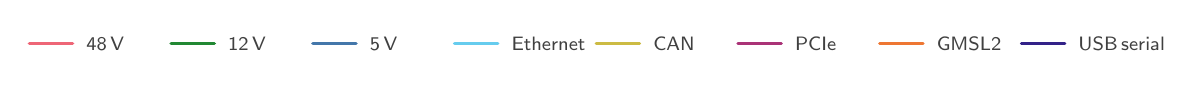
\begin{tikzpicture}[baseline]
  \foreach \i/\col/\lbl in {%
      0/bus48v/48\,V,  1/bus12v/12\,V,  2/bus5v/5\,V,
      3/buseth/Ethernet, 4/buscan/CAN,
      5/buspcie/PCIe, 6/busgmsl/GMSL2, 7/bususb/USB\,serial}
  {
    \draw[line width=1.2pt, color=\col, line cap=round]
      (\i*1.8, 0) -- ++(0.55,0);
    \node[anchor=west, font=\sffamily\scriptsize, text=black!75]
      at (\i*1.8 + 0.6, 0) {\lbl};
  }
\end{tikzpicture}

\caption{System-level electrical block diagram. Subsystems are grouped by
shaded zones; line colour denotes bus type per the legend.}
\label{fig:electrical-block}
\end{figure}

\subsection*{4.2 Power System}
A 48~V battery is the single power source on the vehicle. As shown in
Figure~\ref{fig:power-tree}, the battery passes through a main switch into
two buck converters: a 12~V / 20~A converter for the motor controllers and
other high-power loads, and a 5~V / 6~A converter for the Teensy~4.1 and
low-power peripherals.

Each rail is split into three independently fused output branches. Per-rail
fusing isolates faults so that a short on one load does not pull down the
rest of the vehicle.

\begin{figure}[h]
\centering
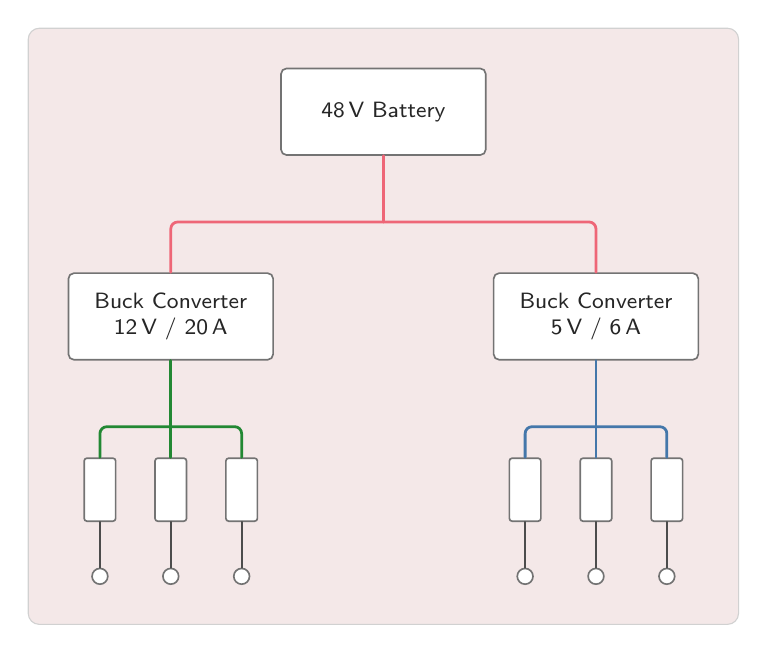
\begin{tikzpicture}[x=1cm, y=1cm]

\node[pblock] (battery2) at (0, 0) {48\,V Battery};
\node[pblock] (buck12p)  at (-2.7, -2.6) {Buck Converter\\12\,V / 20\,A};
\node[pblock] (buck5p)   at ( 2.7, -2.6) {Buck Converter\\5\,V / 6\,A};

\node[fuse] (fL1) at (-3.6, -4.8) {};
\node[fuse] (fL2) at (-2.7, -4.8) {};
\node[fuse] (fL3) at (-1.8, -4.8) {};

\node[fuse] (fR1) at ( 1.8, -4.8) {};
\node[fuse] (fR2) at ( 2.7, -4.8) {};
\node[fuse] (fR3) at ( 3.6, -4.8) {};

\node[term] (oL1) at (-3.6, -5.9) {};
\node[term] (oL2) at (-2.7, -5.9) {};
\node[term] (oL3) at (-1.8, -5.9) {};
\node[term] (oR1) at ( 1.8, -5.9) {};
\node[term] (oR2) at ( 2.7, -5.9) {};
\node[term] (oR3) at ( 3.6, -5.9) {};

% Tinted backdrop for power tree (match Fig 1's power-zone tint)
\begin{scope}[on background layer]
  \node[zone, fill=zoneA,
        fit=(battery2)(buck12p)(buck5p)(fL1)(fR3)(oL1)(oR3)] (z_pt) {};
\end{scope}

% Battery -> two bucks (rounded corners auto)
\coordinate (bsplit) at (0, -1.4);
\draw[buswire, color=bus48v] (battery2.south) -- (bsplit);
\draw[buswire, color=bus48v] (bsplit) -| (buck12p.north);
\draw[buswire, color=bus48v] (bsplit) -| (buck5p.north);

% Buck12 -> 3 fuses (use 12V color)
\coordinate (b12_split) at (-2.7, -4.0);
\draw[buswire, color=bus12v] (buck12p.south) -- (b12_split);
\draw[buswire, color=bus12v] (b12_split) -| (fL1.north);
\draw[buswire, color=bus12v] (b12_split) -- (fL2.north);
\draw[buswire, color=bus12v] (b12_split) -| (fL3.north);

% Buck5 -> 3 fuses (use 5V color)
\coordinate (b5_split) at (2.7, -4.0);
\draw[buswire, color=bus5v] (buck5p.south) -- (b5_split);
\draw[buswire, color=bus5v] (b5_split) -| (fR1.north);
\draw[buswire, color=bus5v] (b5_split) -- (fR2.north);
\draw[buswire, color=bus5v] (b5_split) -| (fR3.north);

% Fuses -> terminals (keep neutral pwire)
\foreach \f/\o in {fL1/oL1, fL2/oL2, fL3/oL3, fR1/oR1, fR2/oR2, fR3/oR3} {
  \draw[pwire] (\f.south) -- (\o.north);
}

\end{tikzpicture}
\caption{Power distribution from the 48~V battery through two buck converters
to fused output rails. Trunk colours match the bus legend of
Figure~\ref{fig:electrical-block}.}
\label{fig:power-tree}
\end{figure}

\subsection*{4.3 Motor Control}
The drivetrain uses two NEO brushless motors, each driven by a SPARK~MAX
motor controller. Both controllers share a single CAN bus to the Teensy~4.1,
which acts as the real-time control node. Each SPARK~MAX reports position
and velocity from its integrated encoder back over the same bus.

The Teensy closes a PID velocity loop per wheel, using encoder feedback from
the SPARK~MAX controllers and reference velocities published by the Jetson
over USB serial. Because the motor controllers, the encoders, and the
microcontroller all live on one CAN bus, no separate signal wiring between
the motor controllers and the Teensy is required.

The hardware emergency stop interrupts the SPARK~MAX supply directly. When
triggered, both controllers lose power and the motors coast to a stop;
software is not in the loop.

\subsection*{4.4 Sensing}
The vehicle uses three classes of sensor:

\begin{itemize}
  \item \textbf{Stereo cameras} — three ZED~X cameras connected to a ZED~Link
    Quad over GMSL2. The ZED~Link Quad attaches to the Jetson over PCIe,
    keeping the cameras off the Ethernet network.
  \item \textbf{LiDAR} — a Velodyne LiDAR provides 3D point clouds for
    obstacle detection and mapping. It reports to the Jetson over Ethernet
    through the on-board router.
  \item \textbf{GPS / IMU} — an Xsens module provides position and
    orientation. It connects directly to the Jetson.
\end{itemize}

Camera, LiDAR, and GPS streams are time-aligned on the Jetson before being
consumed by perception and localization.

\subsection*{4.5 Network and Computation}
The Jetson~Orin is the primary computation unit. It runs perception, sensor
fusion, and trajectory generation, and publishes wheel velocity commands to
the Teensy.

An on-board router carries Ethernet between the Jetson and the Velodyne LiDAR.
The Teensy~4.1 connects to the Jetson via USB serial (115200 baud) rather than
Ethernet. The high-bandwidth camera link is kept separate: the
ZED~Link Quad attaches directly to the Jetson over PCIe so that the three
ZED~X feeds do not contend for the Ethernet network. The Xsens GPS connects
directly to the Jetson.

The same router also exposes a Wi-Fi link to a remote laptop for monitoring,
data capture, and remote shutdown during testing.

\end{document}
